\chapter{Aerospace Applications of SMAs}
\begin{multicols}{2}

The use of Shape Memory Alloys in different fields of engineering is prevalent, and the aerospace sector is no exception \cite{costanza2020shape}. SMAs are used in a wide variety of different aerospace applications for both aeronautical engineering and spaceflight, a few of which are discussed here. The central question in the aeronautical case is how to create aircraft that are more efficient in terms of flight capabilities and overall performance under any sort of flight conditions encountered. Somewhat in contrast and perhaps more exciting, the central question in the spaceflight case is how to create spacecraft that are capable of long distance space travel in order for humans to not only learn about the universe vicariously through rovers and telescopes, but to travel into deep space ourselves and leave the Earth for good. In both cases, SMA’s play key roles in attempting to find solutions to these central questions as will be discussed in this section.

\section{Wing Morphing}

Commercial flights are one of the most widely used modes of transportation in today’s world, especially when it comes to long distance travel. Airplanes rely on a combination of Newton’s laws of motion and Bernoulli’s principle in order to fly. Newton would say that there is a force of gravity pulling the airplane downward and therefore, if the plane wants to fly, there must be an opposing force that is greater than the force of gravity in the upward direction. This is called the \textit{lift} force. An airplane generates a lift force thanks to its high speed and the shape of its wings. The \textit{Camber} of a wing, loosely defined as the overall curvature or shape of the wing, is constructed in such a way to create a pressure difference between the air flowing on the top of the wing versus the air flowing underneath the wing, with the latter having a greater pressure than the former. Since there is more pressure from air flow underneath the wing than on top of the wing, there will be a lift force in the upward direction. Hence, the airplane can fly. However, airplanes face different flight conditions depending on a wide range of different factors such as where they are flying, what altitude they are at and how fast they are moving through the atmosphere. Wing morphing is the idea that the camber or shape of the wing is able to change by means of actuators, based on the different flight conditions the plane faces. This ensures that the flight is more aerodynamically efficient by maximizing the lift to drag ratio. In other words, by controlling the camber of a wing, airplanes are able to maximize their lift force and minimize their drag due to air resistance \cite{barbarino2011review}.

\begin{figure}[H]
    \centering
    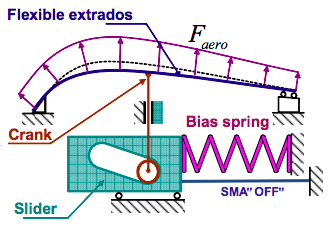
\includegraphics[scale=0.45]{._figures/SMA_Wing_Morphing_Diagram.png}
    \caption[Schematic of wing morphing system on an aircraft wing]{Schematic of wing morphing system on an aircraft wing. The shape of the flexible extrados changes depending on the position of the SMA slider \cite{brailovski2010sma}.}
    \label{fig:wing_morphing}
\end{figure}

In recent years, shape memory alloys were found to be one of the best materials for actuators used in aircraft to achieve camber control. The airfoil of a wing is defined as the cross-sectional shape of a wing. Changes in the camber of the airfoil are controlled by two SMA actuators located inside the wing itself. Figure \ref{fig:wing_morphing} shows the mechanism that controls the camber of the airfoil and all its subsystems, including the SMA actuators. The SMA actuator is connected, via the bias spring, to the slider which in turn is connected to a crank. When the SMA is not active, the bias spring extends and pushes the slider and crank into their nominal position in the wing. Aerodynamic forces then force the flexible extrados, which are defined as the outer layers of the skin of the wing, upward \cite{brailovski2010sma}. When the aircraft is subjected to certain flight conditions, such as changes in temperature and atmospheric pressure, the SMA is activated and causes the bias spring to compress. This pulls the slider and crank to the right and changes the shape of the flexible extrados and hence morphs the wing into a different shape \cite{brailovski2010sma}. This mechanism for camber control, which is based on using SMAs for actuators, provides a way for airplanes to adapt to any variable aerodynamic forces and flight conditions and will in turn improve the efficiency of air travel in the future. 

%\section{Low-Shock Release Mechanisms}

%Spacecrafts are often used to carry certain payloads into orbit around the Earth, or somewhere else in the Solar System. The idea is that the payload is attached to the spacecraft while on Earth and then released from the spacecraft once it reaches its destination. For example, the Cassini/Huygens mission to study the planet Saturn involved the Huygens probe being released from the Cassini spacecraft, which was orbiting Saturn. The Huygens probe then made its journey to one of Saturn’s moons called Titan, while Cassini continued to study Saturn. For many years, pyrotechnic release mechanisms were the dominant type of mechanism used for payload release. However, it was found that these release mechanisms lead to shock failures and in some cases these failures resulted in missions being aborted.\cite{godard2003design} When the payload gets released from the spacecraft, there is a momentary shock that runs through the spacecraft due to the release mechanism. Pyrotechnic shocks are characterized by their high frequency and short duration that run through the spacecraft. These high frequency shocks can lead to the failure of spacecraft hardware. It is for this reason why low-shock release mechanisms on spacecraft are required to increase the probability of a successful mission. 

%Shape memory alloys can be used for low-shock release mechanisms due to their slow actuation time from gradual heating. Before the payload is released, the SMA in the separation device is strained to a low temperature martensite configuration. By slowly heating up the SMA element to its transition temperature via an electrical current, the release mechanism becomes activated and the spacecraft is able to release its payload. This method of payload release eliminates the shock that was present in the pyrotechnic release device because of the slow actuation of the SMA. Release devices based on SMA components have already been used on both mid-sized and micro-sized satellites.\cite{willey2001design} In the case of the micro-sized satellites, there is a need to construct more compact SMA release devices and the endeavor to create these devices has led to the popular \textit{Qwkut}.\cite{peffer2000development} In this device, the SMA component is deformed and detwinned before it is installed on the satellite. Once the satellite is in orbit, the component is heated up recovering its original shape and triggering the release mechanism. 

%One interesting example of a release mechanism that makes use of SMA's is the so called \textit{Micro Sep-Nut}. This mechanism uses a single SMA spring that has been formed into a circular shape. The mechanism is set by inserting a bolt through a housing and then through the inside of the circular SMA spring. See figure \ref{fig:micro-nut} for a diagram of the various components. The cap is then put in place to hold the SMA spring inside the housing. Through manual compression, the SMA spring is compressed from two different sides securing it around the bolt. The release mechanism is now set. 

%\begin{figure}[H]
%    \centering
%    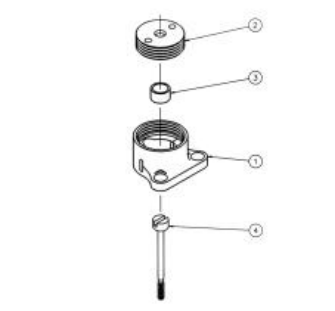
\includegraphics[scale=0.43]{._figures/Micro sep-nut.png}
%    \caption[Diagram of the Micro Sep-Nut assembly]{Diagram of the Micro Sep-Nut assembly. The bottom piece is the bolt. The lower middle piece is the housing. The upper middle piece is the SMA circular spring. The upper-most piece is the cap. Retrieved from \cite{huett2000design}.}
%    \label{fig:micro-nut}
%\end{figure}

%The Micro Sep-Nut is activated for release by heating up the housing that surrounds the SMA spring holding the bolt. As the housing is heated, the SMA spring gets heated and returns to its original circular shape, releasing the bolt. SMA based release mechanisms such as this one will certainly lead to more successful future aerospace missions. 

\section{Mars Rover Tires}
Recently, nitinol has been used in prototypes of a spring tire for future Mars rovers \cite{nasa_2017}. Current rovers make use of solid aluminium wheels which can be punctured by sharp rocks over time. The SMA spring tires were hence developed by NASA Glenn laboratories to make a long-lasting tire capable of withstanding the rough Martian surface. The spring tire exploits the pseudoelastic property of the SMA and the durability of the nitinol alloy. It is strong enough to support the 900 kg rover while deforming to roll smoothly over the terrain. Weight was also a key consideration due to the increased launch cost. The spring tires are relatively light compared to their solid counterparts, weighing in at just a few kilograms each. Hence, this advancement shows promise in helping to extend the lifetime and durability of future Mars rovers.

\section{Solar Sail}
In 1608, German astronomer Johannes Kepler observed a phenomenon that was quite unusual to him at the time. While observing a comet passing by the Sun, he noticed that the comet’s tails were slightly displaced, as if they were blowing in the wind. He hypothesized that the comet’s tails were indeed being blown by what he called ``solar breeze”. Influenced by this astonishing discovery, Kepler thought that one day we would be able to create ships with sails capable of riding this solar breeze, just as ordinary ships with sails ride the breeze of air on Earth. Of course, we know today that Kepler was correct and that the Sun does indeed give off solar wind in the form of charged particles. However in 1873, James Clerk Maxwell showed that sunlight itself could be used as a form of wind for a cosmic ship to use as propulsion. He demonstrated that particles of light, known as photons, exert a small amount of pressure when they collide with an object. This was later experimentally verified by Russian physicist Pyotr Lebedev in 1900 \cite{lebedev1901investigations} and is the basis for how Solar Sails work.

The Solar Sail is a spacecraft that uses the momentum and pressure of solar photons as its mechanism for propulsion. Unlike regular propulsion methods that mix fuel and oxidizer together in a combustion reaction, the Solar Sail takes advantage of solar photons that collide with its sails after they are deployed, which accelerates the spacecraft towards its destination. Figure \ref{fig:solar_sail} is a depiction of what a Solar Sail spacecraft looks like. Because each photon only exerts a small amount of pressure on the sail, the sail itself must be quite large in order to have a high degree of propulsion. The method of deploying the sails has been a difficult challenge for engineers and scientists to overcome. There are limits to certain mechanisms of sail deployment such as high weight and overall complexity of deploying such large sails. In order to maximize the performance of the Solar Sail, it is crucial to have a deployment system that is lightweight and more efficient. Recently, experiments have shown that NiTi wires could be used as actuators for sail deployment, and would be effective in doing so \cite{bovesecchi2019novel}.

\begin{figure}[H]
    \centering
    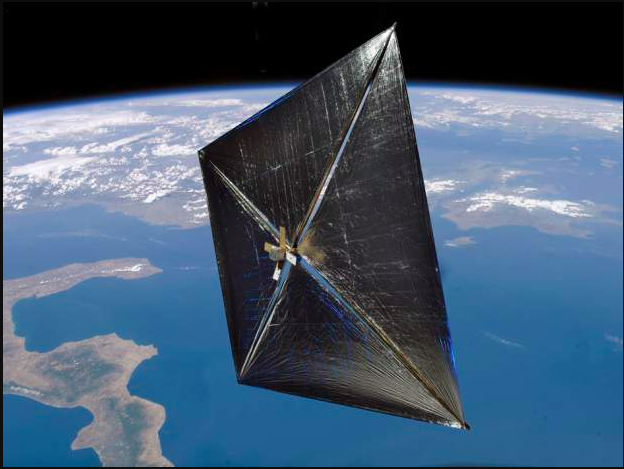
\includegraphics[scale=0.25]{._figures/solar sail.png}
    \caption[Depiction of the Solar Sail spacecraft]{Depiction of the Solar Sail spacecraft. Retrieved from
    \url{https://www.nasa.gov/mission\_pages/tdm/solarsail/index.html}}
    \label{fig:solar_sail}
\end{figure}

As shown in figure \ref{fig:Wire_configs}, small SMA wires made from NiTi are attached to the surface of the sail in certain configurations. The wires are then cooled down to their martensite phase, where they deform in such a way as to fold the sail up before deployment. Once the spacecraft is in space, heat from the Sun activates the SMA wires and they begin to deform back to their original austinsite phase. In doing so, the sails begin to deploy and open up and the spacecraft is ready to begin its journey through the Solar System.

The Solar Sail is an exciting part of the future of space exploration and travel, especially in its exploitation of an essentially inexhaustible fuel source. In the words of Carl Sagan: ``\textit{We have lingered long enough on the shores of the cosmic ocean. We are ready at last to set sail for the stars.}"

\begin{figure}[H]
    \centering
    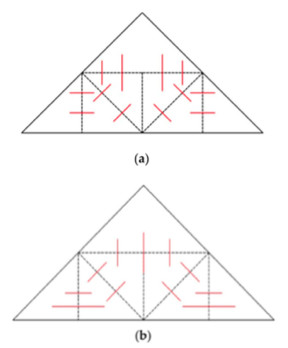
\includegraphics[scale=0.38]{._figures/SMA wire configs.png}
    \caption[SMA wire configurations for solar sail deployment]{Two different SMA wire configurations for sail deployment. The red lines represent the wires. Retrieved from \cite{bovesecchi2019novel}.}
    \label{fig:Wire_configs}
\end{figure}



\end{multicols}